\documentclass[border=6pt]{standalone}
\usepackage{fontspec,unicode-math}
\setmainfont{Noto Sans}
\setsansfont{Noto Sans}
\setmathfont{STIXTwoMath-Regular.otf}
\usepackage{tikz}
\usetikzlibrary{arrows.meta,calc,intersections,patterns,decorations.markings}
\definecolor{ScienceInk}{HTML}{000000}
\definecolor{ScienceCurve}{HTML}{000000}
\definecolor{ScienceAlt}{HTML}{A36035}
\tikzset{axis/.style={draw=ScienceInk,line width=.68pt,>=Latex},
 trace/.style={draw=ScienceCurve,line width=1.42pt,line cap=round,line join=round},
 secondary/.style={draw=ScienceAlt,line width=1.25pt,dashed,line cap=round},
 energy/.style={draw=ScienceInk,line width=1.35pt,line cap=round},
 shiftline/.style={draw=ScienceAlt,densely dashed,line width=1.1pt},
 photon/.style={->,draw=ScienceCurve,line width=1.10pt,>=Latex},
 lab/.style={text=ScienceInk,font=\fontsize{13}{16}\selectfont,inner sep=1.5pt},
 smalllab/.style={text=ScienceInk,font=\fontsize{11}{14}\selectfont,inner sep=1pt},
 panellab/.style={font=\fontsize{13}{16}\itshape,text=ScienceInk,inner sep=0pt}}
\begin{document}


% Figure 7.1: identical shared qenergy gives E+(x)-E0=-(E-(x)-E0).
% The earlier CP05 file added an arbitrary ±0.36 vertical offset and violated the
% text's exactly symmetric dressed quasienergy pair. E0=2.48 is only page layout.
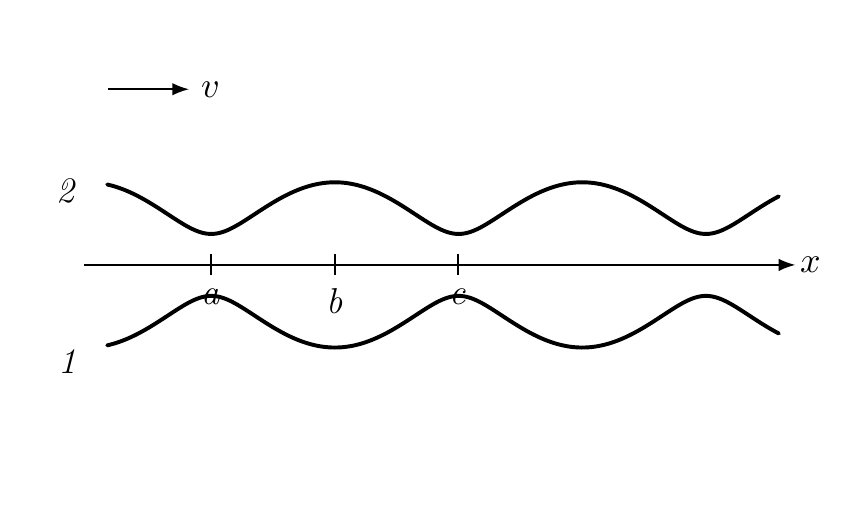
\begin{tikzpicture}[x=1cm,y=1.15cm]
 \path[use as bounding box] (0,0) rectangle (10.3,5.10);
 \def\Delta{.38}\def\Omega{.94}
 \pgfmathdeclarefunction{qenergy}{1}{\pgfmathparse{sqrt(\Delta*\Delta+\Omega*\Omega*cos(deg(#1))^2)}}
 \draw[axis,->] (.72,2.48)--(9.75,2.48) node[lab,anchor=west] {$x$};
 \draw[trace,smooth,variable=\x,domain=.25:8.78,samples=270]
    plot ({.76+\x},{2.48+.90*qenergy(\x)});
 \draw[trace,smooth,variable=\x,domain=.25:8.78,samples=270]
    plot ({.76+\x},{2.48-.90*qenergy(\x)});
 \foreach \pos/\lab in {2.33/a,3.90/b,5.47/c}{
   \draw[axis] (\pos,2.37)--(\pos,2.60);
   \node[lab,anchor=north] at (\pos,2.27) {$\mathit{\lab}$};
 }
 \node[lab,anchor=east] at (.68,3.30) {$\mathit{2}$};
 \node[lab,anchor=east] at (.68,1.41) {$\mathit{1}$};
 \draw[axis,->] (1.02,4.42)--(2.05,4.42);
 \node[lab,anchor=west] at (2.15,4.42) {$v$};
\end{tikzpicture}

\end{document}
